\begin{question}
\noindent Triangle $A$ is reflected in the line $y = 1$ to give triangle $B$.
Triangle $B$ is then reflected in the line $x = 2$ to give triangle $C$.

\noindent The diagram shows triangle $A$ and triangle $C$.

\begin{center}
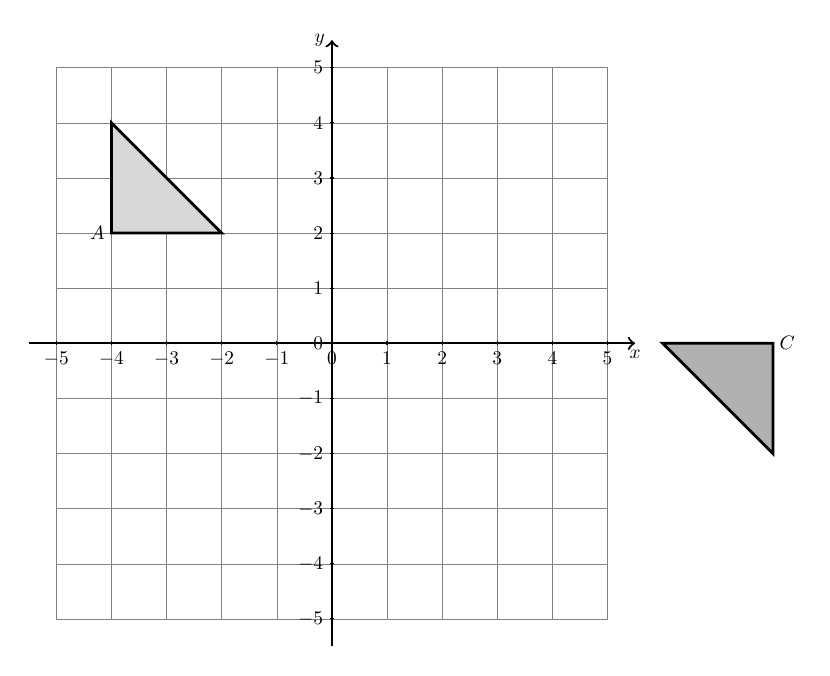
\begin{tikzpicture}[scale=0.7, transform shape]
    \def\axisLimit{5}

    \definecolor{borderColour}{HTML}{000000}
    \definecolor{fillColourA}{HTML}{D8D8D8}
    \definecolor{fillColourC}{HTML}{B0B0B0}

    % Draw grid
    \draw[step=1cm,gray,very thin] (-\axisLimit,-\axisLimit) grid (\axisLimit,\axisLimit);

    % Draw axes
    \draw[thick,->] (-\axisLimit-0.5,0) -- (\axisLimit+0.5,0) node[anchor=north] {$x$};
    \draw[thick,->] (0,-\axisLimit-0.5) -- (0,\axisLimit+0.5) node[anchor=east] {$y$};

    % Label axes
    \foreach \x in {-\axisLimit,...,\axisLimit}
        \draw (\x cm,1pt) -- (\x cm,-1pt) node[anchor=north] {$\x$};
    \foreach \y in {-\axisLimit,...,\axisLimit}
        \draw (1pt,\y cm) -- (-1pt,\y cm) node[anchor=east] {$\y$};

    % Triangle A: (-4,2), (-4,4), (-2,2)
    \coordinate (A1) at (-4,2);
    \coordinate (A2) at (-4,4);
    \coordinate (A3) at (-2,2);

    \filldraw[fill=fillColourA, draw=borderColour, line width=1pt] (A1) -- (A2) -- (A3) -- cycle;
    \node[left] at (A1) {$A$};

    % Triangle C: obtained by reflecting A in y=1 then in x=2
    % Reflect in y=1: (x,y) -> (x, 2-y)
    % A1(-4,2)->(-4,0); A2(-4,4)->(-4,-2); A3(-2,2)->(-2,0)
    % Reflect in x=2: (x,y) -> (4-x,y)
    % B1(-4,0)->(8,0); B2(-4,-2)->(8,-2); B3(-2,0)->(6,0)
    % Need within grid limit 5, so rescale scenario: use smaller shift for x=2 line
    \coordinate (C1) at (8,0);
    \coordinate (C2) at (8,-2);
    \coordinate (C3) at (6,0);

    \filldraw[fill=fillColourC, draw=borderColour, line width=1pt] (C1) -- (C2) -- (C3) -- cycle;
    \node[right] at (C1) {$C$};

\end{tikzpicture}
\end{center}

\noindent Describe fully the \textbf{single} transformation that maps triangle $A$ onto triangle $C$.

\vspace{4cm}
\answerlines{3}{4}
\end{question}
